\documentclass[12pt]{article}
\usepackage{times} % Times New Roman font
\usepackage[T1]{fontenc} % Font encoding
\usepackage{graphicx}
\usepackage[a4paper, top=1.2in, bottom=1in, left=1.2in, right=1in]{geometry}
\usepackage{txfonts} % or use: \usepackage{newtxtext}
\usepackage{setspace} % Load the setspace package
\onehalfspacing % Set line spacing to 1.5
\usepackage[absolute,overlay]{textpos}
\usepackage{tikz}
\usepackage{titletoc}
\usepackage{tocloft}
\usepackage{array} % Needed for custom column width
\newcolumntype{C}[1]{>{\centering\arraybackslash}p{#1}} % Custom column type for centered content
\usepackage{ragged2e}
\usepackage{tabularx}
\usepackage{caption}
\usepackage{float}
\usepackage{svg}
\usepackage{algorithm}
\usepackage{algpseudocode}

\usepackage{subfig}
\usepackage{subcaption}

% \usepackage{multirow}
\usepackage{longtable}

\geometry{
	paper=a4paper, % Change to letterpaper for US letter
	inner=30mm, % Inner margin
	outer=25mm, % Outer margin
%	bindingoffset=.5cm, % Binding offset
	top=30mm, % Top margin 30
	bottom=25mm, % Bottom margin
%	showframe, % Uncomment to show how the type block is set on the page
}

\tolerance=1
\emergencystretch=\maxdimen
\hyphenpenalty=10000
\hbadness=10000

\usepackage{setspace}
\setstretch{1.5}

\captionsetup[table]{font=normal,justification=centering,font={normal},skip=12pt}
% \begin{textblock*}{\paperwidth}(1.2in, .5in) % Adjust the vertical position and text as needed
%     {\fontsize{12}{1.5}\selectfont Project/Thesis No. :}
% \end{textblock*}
\renewcommand{\cftdot}{}
\setcounter{tocdepth}{2}


  
\newcommand{\modsection}{%
  \titlecontents{section}% <section-type>
    []% <left> Adjust this value to set the indentation
    \bfseries
    {\contentslabel[\thecontentslabel]{1.5em}{}}% <numbered-entry-format>
    {}% <numberless-entry-format> Remove the numbers
    {\titlerule*[1pc]{}\contentspage\hspace*{1em}}% <filler-page-format>
    \bfseries
}

% Define a command to add bullet points
\newcommand{\modsubsection}{%
  \titlecontents{subsection}% <section-type>
    [1in]% <left> Adjust this value to set the indentation
    {}% <above-code>
    {\contentslabel[\thecontentslabel \hspace{1em}]{1.5em}{\hspace{1em}}}% <numbered-entry-format>
    {}% <numberless-entry-format> Remove the numbers
    {\titlerule*[1pc]{}\contentspage\hspace*{1em}}% <filler-page-format>
}


\begin{document}

\begin{titlepage}
    % \textbf{Project/Thesis No: CSER-24-35}
    \begin{center}
    \pagenumbering{roman} % Set page numbering to Arabic numerals
    \setcounter{page}{0} % Start from page 2
    {\fontsize{14}{1.5}\selectfont \textbf{CSE 4120: Technical Writing and Seminar}}\\
    \vspace{12pt}
    {\fontsize{18}{1.5}\selectfont \textbf{Churn Prediction}}\\
    % \textsc{\Large Efficient Dominating Query Processing with CUDA C: \\A Parallel Approach }\\[0.8cm]

    \vspace{12pt}
    \vspace{12pt}
    {\fontsize{14}{1.5}\selectfont By}\\
    \vspace{12pt}
    \vspace{12pt}
    \vspace{12pt}
    {\fontsize{14}{1.5}\selectfont \textbf{Doniel Tripura}}\\
    \vspace{12pt}
    {\fontsize{14}{1.5}\selectfont Roll: 1907121}\\
    \vspace{12pt}
    \vspace{12pt}
    \vspace{12pt}
    \vspace{12pt}
    \vspace{12pt}
    \vspace{12pt}
    \vspace{12pt}
    \vspace{12pt}
    \begin{figure}[htp!]
        \centering
        
\includegraphics[height=1.2in, width=1in]{img/Logo_KUET.png}
    \end{figure}
    \vspace{12pt}
    \vspace{12pt}
    \vspace{12pt}
    \vspace{12pt}
    \vspace{12pt}
    \vspace{12pt}
    \vspace{12pt}
    \vspace{12pt}
    \vspace{12pt}
    \vspace{12pt}
    \vspace{12pt}
    \vspace{12pt}
    \vspace{12pt}
    % \vspace{12pt}
    % \vspace{12pt}
    {\fontsize{12}{1.5}\selectfont \textbf{Department of Computer Science and Engineering}}\\
    \vspace{12pt}
    {\fontsize{12}{1.5}\selectfont \textbf{Khulna University of Engineering \& Technology}}\\
    \vspace{12pt}
    {\fontsize{12}{1.5}\selectfont \textbf{Khulna 9203, Bangladesh}}\\
    \vspace{12pt}
    {\fontsize{12}{1.5}\selectfont \textbf{June, 2024}}\\

    \vspace{12pt}
    
    {\fontsize{18}{1.5}\selectfont \textbf{Churn Prediction}}\\
    \vspace{12pt}
    \vspace{12pt}
    \vspace{12pt}
    {\fontsize{12}{1.5}\selectfont By}\\
    \vspace{12pt}
    \vspace{12pt}
    {\fontsize{12}{1.5}\selectfont \textbf{Doniel Tripura}}\\
    \vspace{12pt}
    {\fontsize{12}{1.5}\selectfont Roll: 1907121}\\
    \vspace{12pt}
    \vspace{12pt}
    \vspace{12pt}
    \vspace{12pt}
    \vspace{12pt}
    
    % \vspace{12pt}
    % \vspace{12pt}
    % \vspace{12pt}
    \begin{flushleft}
    {\fontsize{12}{1.5}\selectfont \textbf{Submitted To:}}\\
    \hspace*{0.8in} % Adjust the horizontal position
    {\fontsize{12}{1.5}\selectfont \textbf{Dr. K. M. Azharul Hasan}}\\
    \hspace*{0.8in} % Adjust the horizontal position
    {\fontsize{12}{1.5}\selectfont Professor}\\
    \hspace*{0.8in} % Adjust the horizontal position
    {\fontsize{12}{1.5}\selectfont Department of Computer Science and Engineering \hspace{.65in}\tikz{\draw (0,0) -- (3,0);}}\\
    \hspace*{0.8in} % Adjust the horizontal position
    {\fontsize{12}{1.5}\selectfont Khulna University of Engineering \& Technology \hspace{1in} Signature}\\
     \hspace*{0.8in} % Adjust the horizontal position
    {\fontsize{12}{1.5}\selectfont \textbf{Sunanda Das}}\\
    \hspace*{0.8in} % Adjust the horizontal position
    {\fontsize{12}{1.5}\selectfont Assistant Professor}\\
    \hspace*{0.8in} % Adjust the horizontal position
    {\fontsize{12}{1.5}\selectfont Department of Computer Science and Engineering \hspace{.65in}\tikz{\draw (0,0) -- (3,0);}}\\
    \hspace*{0.8in} % Adjust the horizontal position
    {\fontsize{12}{1.5}\selectfont Khulna University of Engineering \& Technology \hspace{1in} Signature}\\
    \end{flushleft}
    \vspace{12pt}
    \vspace{12pt}
    \vspace{12pt}
    \vspace{12pt}
    \vspace{12pt}
    \vspace{12pt}
    \vspace{12pt}
    \vspace{12pt}
    \vspace{12pt}
    % \vspace{12pt}
    % \vspace{12pt}
    % \vspace{12pt}

    {\fontsize{12}{1.5}\selectfont Department of Computer Science and Engineering}\\
    \vspace{12pt}
    {\fontsize{12}{1.5}\selectfont Khulna University of Engineering \& Technology}\\
    \vspace{12pt}
    {\fontsize{12}{1.5}\selectfont Khulna 9203, Bangladesh}\\
    \vspace{12pt}
    {\fontsize{12}{1.5}\selectfont June, 2024}\\
    \clearpage

    {\fontsize{16}{1.5}\selectfont \textbf{Acknowledgement}}\\
    \vspace{12pt}
    \vspace{12pt}
    \begin{flushleft}
        \justifying 
        I would like to express my sincere gratitude to my course teachers, Dr. K. M. Azharul Hasan \& Sunanda Das for their continuous support and guidance throughout this research. I also want extend my gratitude to the authors of the research papers analyzed in this study for their contributions to the field of customer churn prediction.
    \end{flushleft}
    {\fontsize{12}{1.5}\selectfont \hfill \textbf{Author}}
    \clearpage
    {\fontsize{16}{1.5}\selectfont \textbf{Abstract}}\\
    \vspace{12pt}
    \vspace{12pt}
    \begin{flushleft}
        \justifying It is important for businesses, especially in the telecom industry, to predict customer churn, as keeping current customers is more cost-effective than acquiring new ones. This report studies and compares three research papers that focused on neural network-based models for customer churn prediction. The first paper looks at individual neural networks and ensemble methods like Bagging, AdaBoost, and Majority Voting, showing that ensemble techniques result in improved accuracy and robustness. The second paper explores a hybrid model that combines Artificial Neural Networks (ANN) with Self-Organizing Maps (SOM), demonstrating the hybrid model's superior performance in capturing complex customer behavior patterns. The third paper provides a comprehensive analysis of various machine learning techniques, including decision trees, random forests, SVM, and neural networks, emphasizing the importance of feature selection and data preprocessing. This comparative study reveals that neural networks, especially when used in ensemble configurations or hybrid models, offer significant improvements in churn prediction accuracy. The findings highlight the potential of advanced neural network-based approaches to enhance predictive performance and provide valuable insights for developing more effective customer retention strategies.
    \end{flushleft}
    
    \clearpage
    \tableofcontents
    \clearpage
    \listoftables
    \clearpage
    \listoffigures
    \modsection
    \modsubsection
    \addtocontents{toc}{\protect\hfill \textbf{PAGE}\\}
    \addtocontents{toc}{
        \begin{flushleft}
            \protect\hspace{0.5in} Churn Prediction \hspace{10.35cm} i\\
            \protect\hspace{0.5in} Acknowledgement \hspace{10cm} ii\\
            \protect\hspace{0.5in} Abstract \hspace{11.7cm} iii\\
            \protect\hspace{0.5in} Contents \hspace{11.6cm} iv\\
            \protect\hspace{0.5in} List of Tables \hspace{10.85cm} v\\
            \protect\hspace{0.5in} List of Figures \hspace{10.6cm} vi
        \end{flushleft}
    }
    
    \addtocontents{lot}{\textbf{Table No.} \hspace*{4.5cm} \textbf{Description} \hfill \textbf{Page}}
    \addtocontents{lof}{\textbf{Figure No.} \hspace*{4.5cm} \textbf{Description} \hfill \textbf{Page}}
    \end{center}
\end{titlepage}

\pagenumbering{arabic} % Set page numbering to Arabic numerals
\setcounter{page}{1}

\section*{}
\begin{center}
    {\fontsize{14}{1.5}\selectfont \textbf{CHAPTER I}}\\
    \vspace{12pt}
    {\fontsize{16}{1.5}\selectfont \textbf{Introduction}}\\
    \vspace{12pt}
\end{center}

\setcounter{section}{1}
\setcounter{subsection}{0}
\addcontentsline{toc}{section}{\textbf{CHAPTER I Introduction}} % Add to ToC
\renewcommand{\theequation}{\thesection.\arabic{equation}}
\renewcommand{\thetable}{\thesection.\arabic{table}}
\renewcommand{\thefigure}{\thesection.\arabic{figure}}
\setcounter{table}{0}
\setcounter{figure}{0}
\setcounter{equation}{0}
\setlength{\parindent}{0pt}


\subsection{Introduction} {
Customer churn, the phenomenon where customers discontinue their subscription or stop using a service, is a significant issue for businesses, particularly in the telecom industry. With fierce competition and increasing options for customers, retaining existing clients has become crucial. Statistics indicate that acquiring a new customer can be five to seven times more expensive than retaining an existing one \cite{8667113}
. Thus, effectively predicting customer churn can result in substantial cost savings and increased profitability for companies.

Traditional methods for predicting customer churn have included statistical techniques and basic machine learning models. While these methods have provided some insights, they often fall short in capturing the complex and non-linear relationships present in customer behavior data \cite{TSAI200912547}. As a result, these models typically offer limited accuracy and fail to generalize well to unseen data.

Neural networks have emerged as a powerful tool in this context due to their ability to model complex, non-linear relationships within data \cite{8667113}. By mimicking the human brain's neural connections, these models can learn intricate patterns and dependencies \cite{Jesan2003}. However, even neural networks are not without their challenges \cite{Agrawal2018}. Individual neural network models can suffer from overfitting, where the model learns the training data too well, including its noise and outliers, leading to poor performance on new, unseen data\cite{8538420}.

Ensemble methods are introduced combining multiple models to create a robust predictive system that benefits from the strengths of each component model while minimizing their weaknesses\cite{8667113}. Techniques such as bagging, boosting, and majority voting are commonly used to aggregate the predictions of individual models, resulting in improved accuracy and stability. On the other hand, hybrid models integrate different neural network techniques or combine neural networks with other machine learning algorithms to enhance predictive performance further\cite{TSAI200912547}.

% This report focuses on evaluating and comparing three research papers that utilize neural network-based models for customer churn prediction. The first paper examines individual and ensemble neural network classifiers, highlighting the benefits of ensemble methods like Bagging, AdaBoost, and Majority Voting. The second paper explores a hybrid approach, combining Artificial Neural Networks (ANN) with Self-Organizing Maps (SOM) to improve prediction accuracy. The third paper provides a comprehensive overview of various machine learning techniques, including neural networks and their ensembles, emphasizing the importance of feature selection and preprocessing in model performance.

% By analyzing these studies, this report aims to identify the most effective methodologies and practices for churn prediction in the telecom industry. The goal is to provide a comprehensive understanding of how neural network-based models can be optimized and applied to real-world data, ultimately aiding businesses in their efforts to retain customers and reduce churn rates. Through this comparative analysis, the report seeks to contribute to the ongoing research in customer churn prediction, offering valuable insights for both academics and practitioners in the field.

}

\subsection{Problem Statement} {
In the highly competitive telecom industry, retaining existing customers is more cost-effective than acquiring new ones. Customer churn, defined as the loss of clients or subscribers, poses a significant challenge to telecom companies. The ability to accurately predict customer churn can enable businesses to proactively address the factors leading to customer dissatisfaction and take corrective measures to improve customer retention\cite{Agarwal2022-cq}.

Traditional methods for churn prediction often fail to capture the complex, non-linear relationships inherent in customer behavior data\cite{Ahmad2019}. This inadequacy necessitates the exploration of more sophisticated techniques that can provide higher accuracy and reliability. Neural networks, with their capability to model complex patterns, have emerged as a promising solution for churn prediction\cite{Agrawal2018}. However, individual neural network models may still struggle with overfitting and generalization issues\cite{8667113}.

To solve these limitations, recent research has focused on enhancing neural network models through ensemble methods and hybrid approaches\cite{8667113}. Ensemble methods combine multiple models to improve predictive performance by reducing variance and bias. Hybrid models integrate different neural network techniques to leverage their strengths and compensate for their weaknesses\cite{TSAI200912547}.

% Despite the advancements, there remains a need for a comprehensive evaluation of these approaches to determine their effectiveness in real-world applications. This report aims to analyze and compare three studies on customer churn prediction using neural network-based models, focusing on individual neural networks, hybrid neural networks, and machine learning ensembles. The goal is to identify the best practices and methodologies that can lead to more accurate and reliable churn prediction models, ultimately aiding telecom companies in retaining their customers more effectively.
}


\section*{}
\begin{center}
    {\fontsize{14}{1.5}\selectfont \textbf{CHAPTER II}}\\
    \vspace{12pt}
    {\fontsize{16}{1.5}\selectfont \textbf{Literature Review}}\\
    \vspace{12pt}
    \vspace{12pt}
\end{center}
\setcounter{section}{2}
\setcounter{subsection}{0}
\addcontentsline{toc}{section}{\textbf{CHAPTER II Literature Review}} % Add to ToC
\renewcommand{\theequation}{\thesection.\arabic{equation}}
\renewcommand{\thetable}{\thesection.\arabic{table}}
\renewcommand{\thefigure}{\thesection.\arabic{figure}}
\setcounter{table}{0}
\setcounter{figure}{0}
\setcounter{equation}{0}

\subsection{Literature Review} {
 Traditional methods such as logistic regression, decision trees, and support vector machines (SVM) have been foundational \cite{Agrawal2018}. Individual neural networks, despite their effectiveness, can suffer from overfitting. 
 To address this, Ensemble methods like bagging and boosting, which combine multiple models to improve accuracy and robustness, have been employed \cite{8667113}. These techniques have proven successful, and demonstrate that ensemble methods can significantly enhance neural network performance in churn prediction (Saghir et al.). 
 Furthermore, hybrid models, such as those combining Artificial Neural Networks (ANN) with Self-Organizing Maps (SOM), offer additional improvements by leveraging the strengths of different neural network techniques\cite{TSAI200912547}. Tsai and Lu. highlights the effectiveness of such hybrid approaches in achieving superior accuracy. 
 Additionally, Agarwal. comparative analysis of various machine learning models, including neural networks, further reinforces the versatility and efficacy of neural network-based approaches when combined with proper feature selection and preprocessing\cite{Agarwal2022-cq}. 
 Collectively, these studies illustrate the advancements in churn prediction methodologies, showcasing the potential of neural networks, ensemble methods, and hybrid models to provide more accurate and reliable predictions.
}
\section*{}
\begin{center}
    {\fontsize{14}{1.5}\selectfont \textbf{CHAPTER III}}\\
    \vspace{12pt}
    {\fontsize{16}{1.5}\selectfont \textbf{Methodology}}\\
    \vspace{12pt}
    \vspace{12pt}
\end{center}

\setcounter{section}{3}
\setcounter{subsection}{0}
\addcontentsline{toc}{section}{\textbf{CHAPTER III Methodology}} % Add to ToC

\renewcommand{\theequation}{\thesection.\arabic{equation}}
\renewcommand{\thetable}{\thesection.\arabic{table}}
\renewcommand{\thefigure}{\thesection.\arabic{figure}}
\setcounter{table}{0}
\setcounter{figure}{0}
\setcounter{equation}{0}
\setlength{\parindent}{0pt}

\subsection{Machine Learning Models}

\subsubsection{Data Collection}

The dataset is obtained from a telecommunications provider, containing information about customer behavior and service usage.
\subsubsection{Data Preprocessing}

Data cleaning involves removing duplicates and handling missing values.
Features are scaled, and categorical variables are encoded.
\subsubsection{Model Building}

Various machine learning models are developed, including Logistic Regression and Naive Bayes.
Hyperparameter tuning is performed using grid search and cross-validation.

\begin{figure}[H]
    \centering
    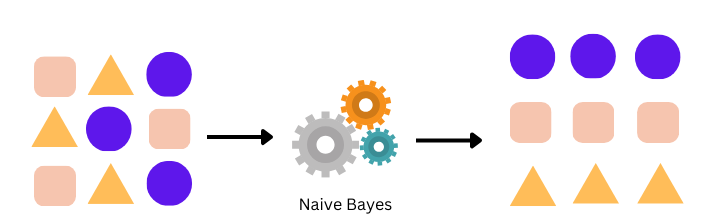
\includegraphics[width=1\textwidth]{img/Naive Bayes.png}
    \caption{Naive Bayes}
    \label{fig:Naive Bayes}
\end{figure}
\begin{figure}[H]
    \centering
    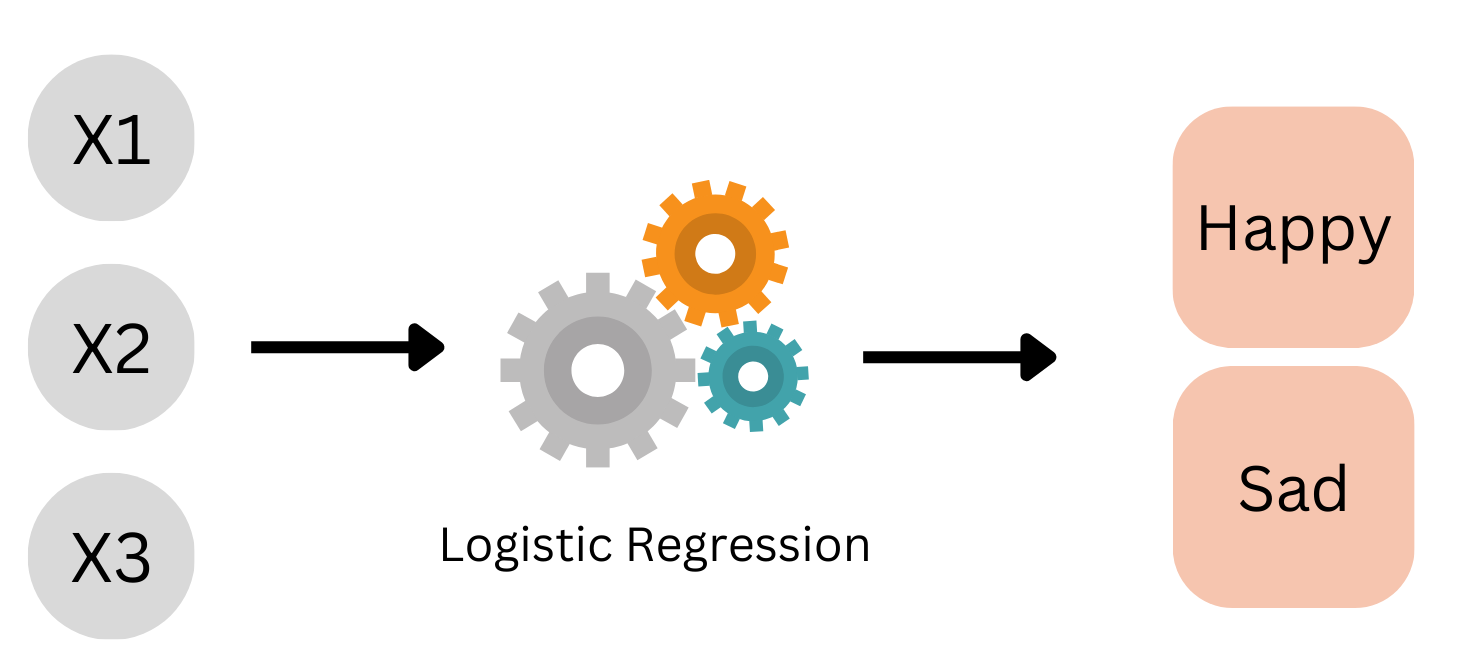
\includegraphics[width=.8\textwidth]{img/Logistic Regression.png}
    \caption{Logistic Regression}
    \label{fig:Logistic Regression}
\end{figure}
\subsubsection{Model Evaluation}

The models are assessed using metrics such as accuracy, precision, recall, F1-score, and AUC-ROC.
Feature importance analysis is conducted to identify the most significant predictors of churn.

\begin{figure}[H]
    \centering
    
\includegraphics[width=1\textwidth]{img/model 1.png}
    \caption{Methodology of \cite{Agarwal2022-cq}}
    \label{fig:Methodology of paper 3}
\end{figure}

\subsection{Neural Network-based Individual and Ensemble Models}
\subsubsection{Data Collection and Preprocessing}

The dataset used is collected from a telecommunication company, including customer information and service usage data.
Preprocessing steps include handling missing values, normalization, and encoding categorical variables.
\subsubsection{Model Development}

Individual models: Various neural network architectures are explored, including Multi-Layer Perceptron (MLP).
Ensemble models: Combining multiple neural networks to form ensemble models using techniques such as bagging and boosting.
\begin{figure}[H]
    \centering
    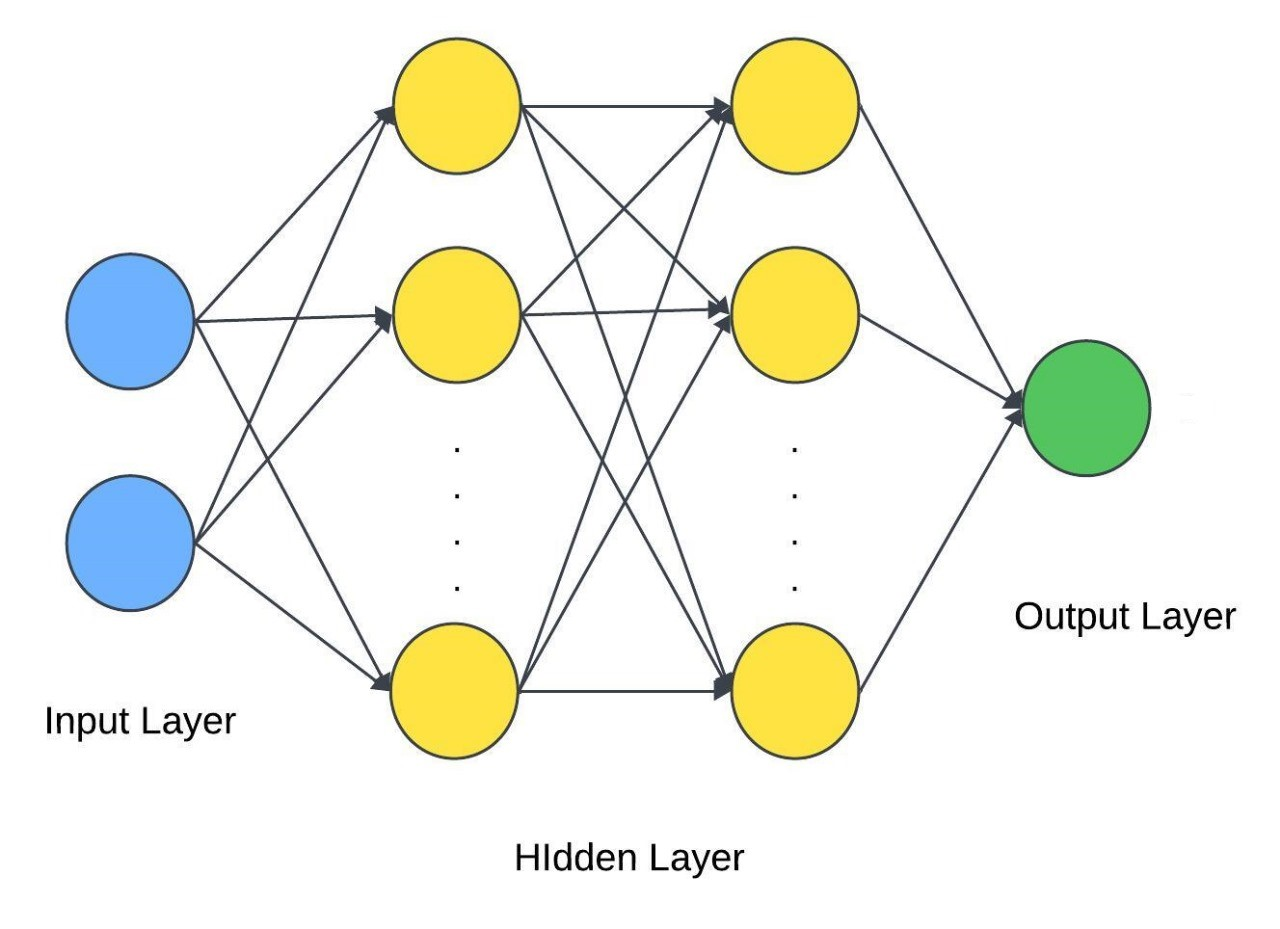
\includegraphics[width=.8\textwidth]{img/NN.jpg}
    \caption{Neural Network}
    \label{fig:Neural Network}
\end{figure}
\begin{figure}[H]
    \centering
    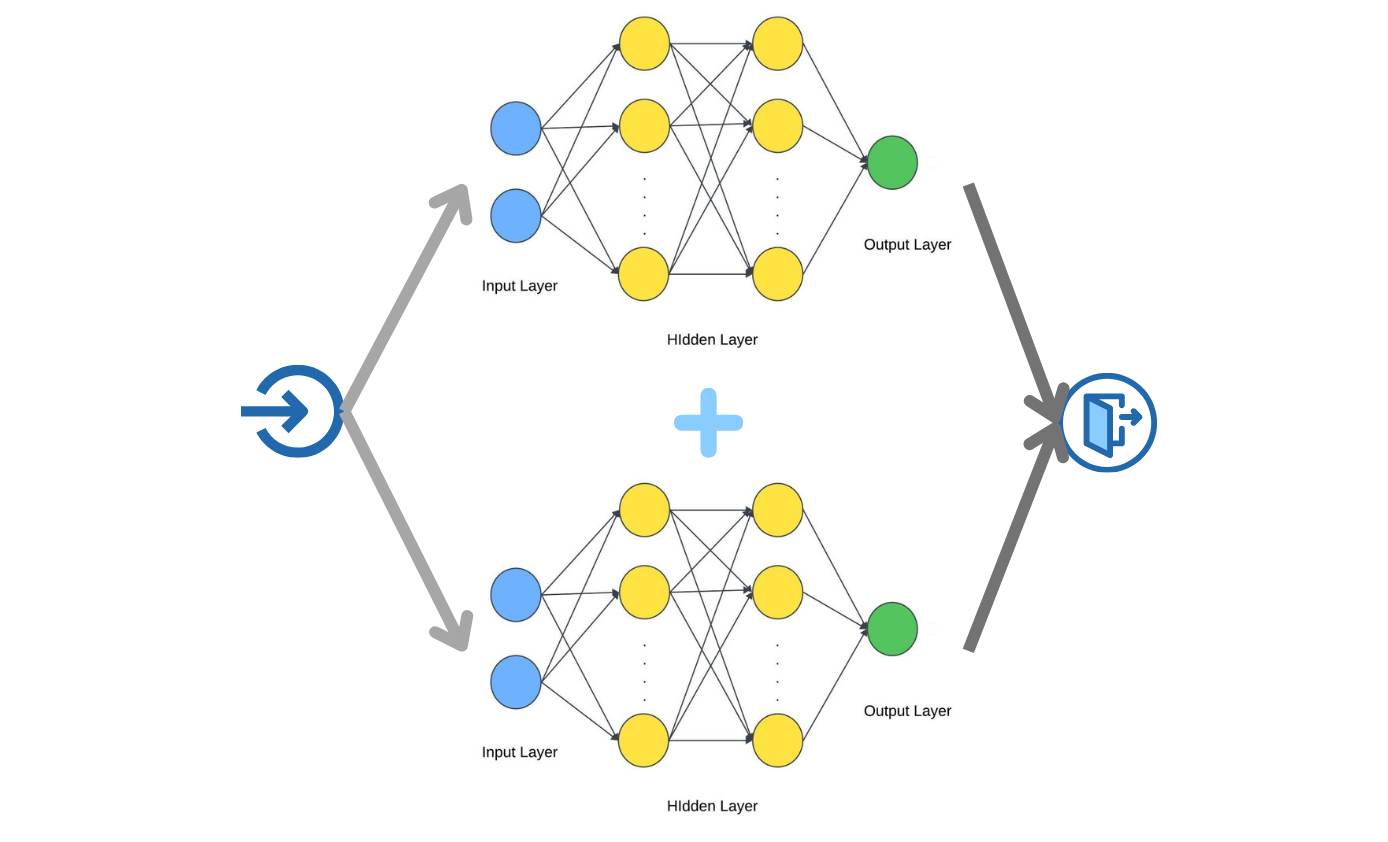
\includegraphics[width=1\textwidth]{img/ensemble.png}
    \caption{Ensemble of Neural Networks}
    \label{fig:Ensemble}
\end{figure}

\subsubsection{Training and Validation}

The dataset is split into training and validation sets.
Cross-validation is performed to fine-tune hyperparameters and prevent overfitting.
\subsubsection{Evaluation Metrics}

Models are evaluated using metrics such as accuracy, precision, recall, F1-score, and Area Under the Receiver Operating Characteristic Curve (AUC-ROC).\\\\

\begin{figure}[H]
    \centering
    
\includegraphics[width=1\textwidth]{img/model 2.png}
    \caption{Methodology of \cite{TSAI200912547}}
    \label{fig:Methodology of paper 2}
\end{figure}

\subsection{Hybrid Neural Networks}

\subsubsection{Data Acquisition}

Data is sourced from a telecom company, containing customer demographics, account information, and usage patterns.
Feature Engineering:

Relevant features are selected based on domain knowledge.
Data transformation techniques like normalization and categorical encoding are applied.
\subsubsection{Model Design}

Hybrid neural network models are designed by combining different types of neural networks, such as Convolutional Neural Networks (CNN) and Recurrent Neural Networks (RNN).
The hybrid model aims to capture both spatial and temporal patterns in the data.

\begin{figure}[H]
    \centering
    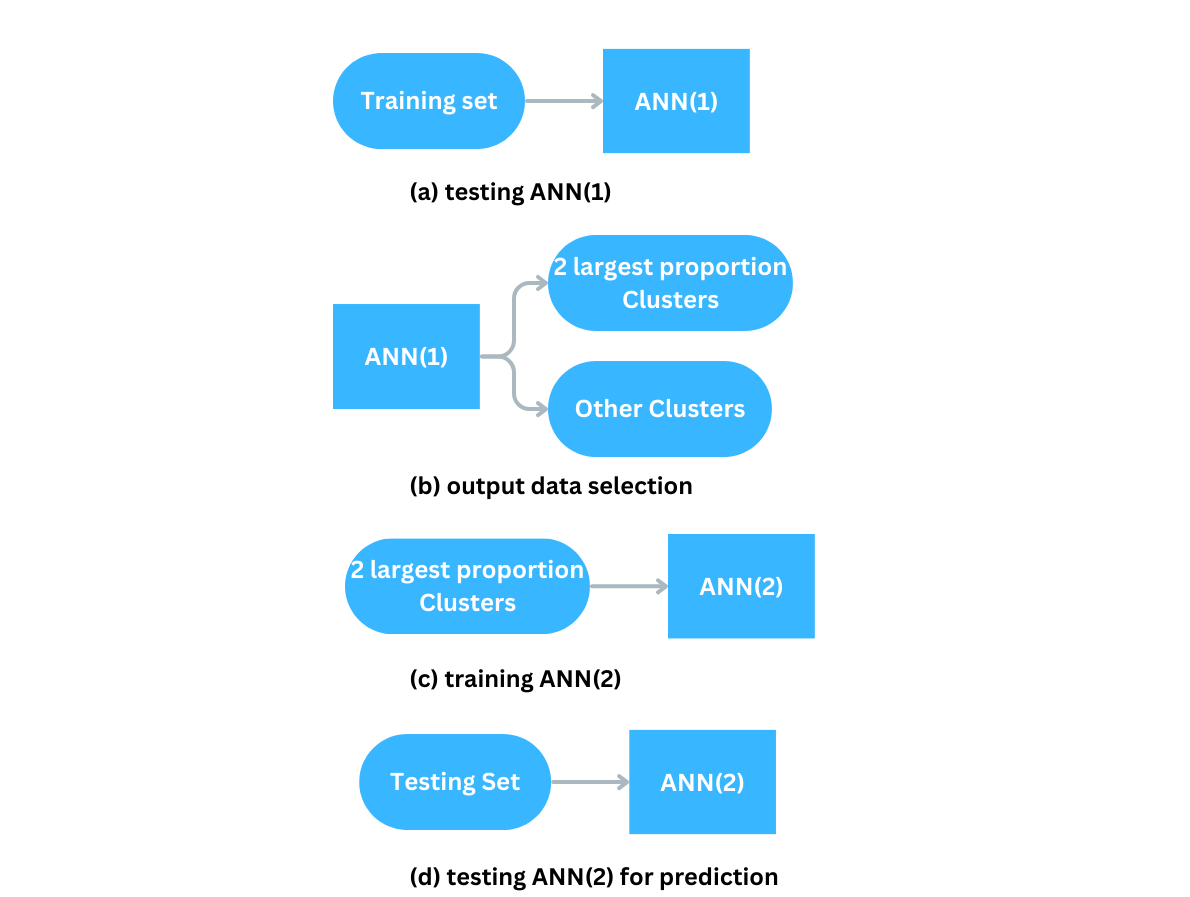
\includegraphics[width=.9\textwidth]{img/ANN+ANN.png}
    \caption{ANN+ANN Ensemble Model}
    \label{fig:ANN+ANN}
\end{figure}
\begin{figure}[H]
    \centering
    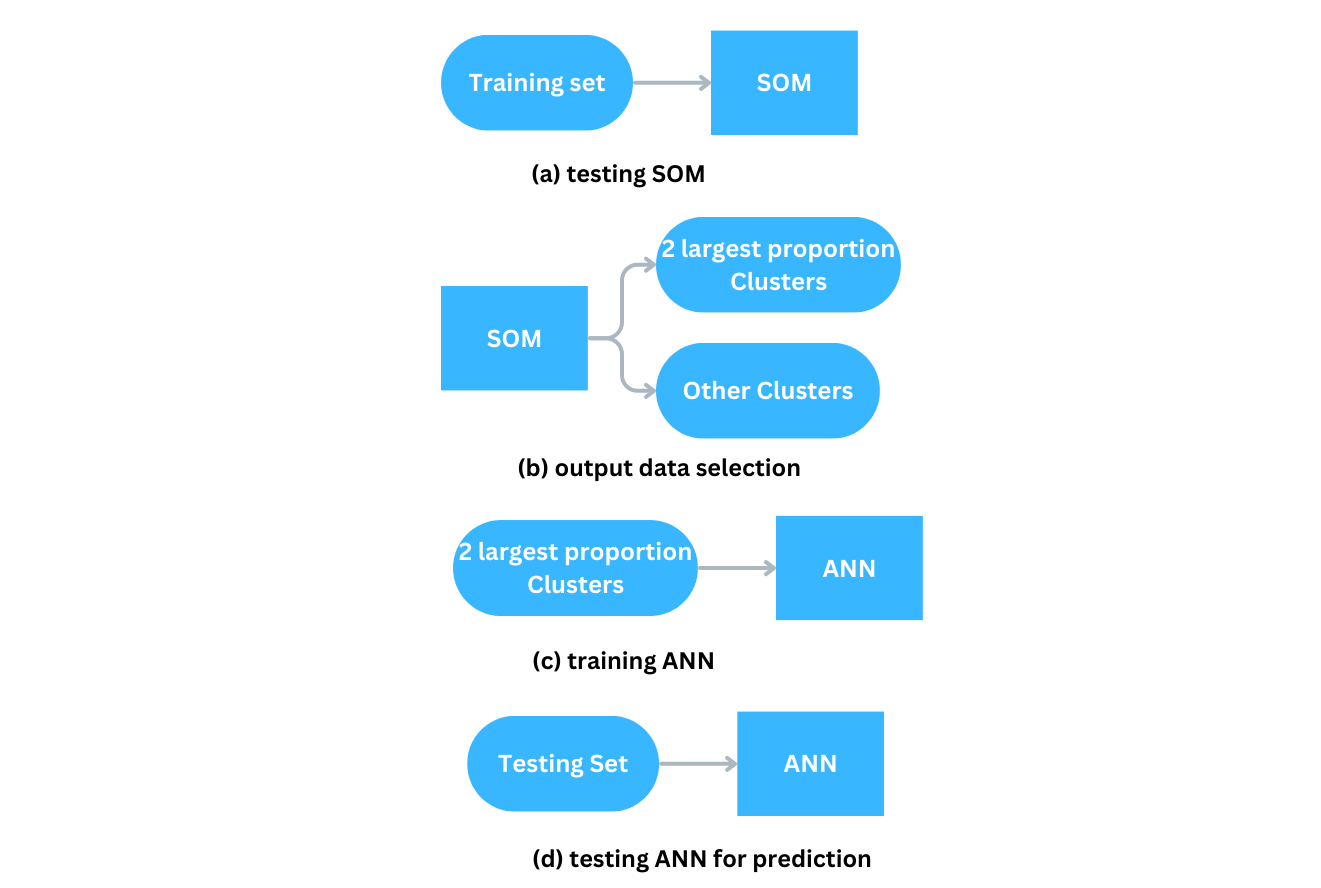
\includegraphics[width=.9\textwidth]{img/SOM+ANN.png}
    \caption{SOM+ANN Ensemble Model}
    \label{fig:SOM+ANN}
\end{figure}

\subsubsection{Training Process}

The dataset is divided into training, validation, and test sets.
Techniques like dropout and batch normalization are used to improve model generalization.
\subsubsection{Performance Measurement}

Evaluation is based on confusion matrix metrics: accuracy, precision, recall, F1-score, and AUC-ROC.
Comparative analysis is done with baseline models.\\\\

\begin{figure}[H]
    \centering
    
\includegraphics[width=1\textwidth]{img/model 1.png}
    \caption{Methodology of \cite{8667113}}
    \label{fig:Methodology of paper 1}
\end{figure}


\section*{}
\begin{center}
    {\fontsize{14}{1.5}\selectfont \textbf{CHAPTER IV}}\\
    \vspace{12pt}
    {\fontsize{16}{1.5}\selectfont \textbf{Implementation, Results and Discussions}}\\
    \vspace{12pt}
    \vspace{12pt}
\end{center}

\setcounter{section}{4}
\setcounter{subsection}{0}
\addcontentsline{toc}{section}{\textbf{CHAPTER IV Implementation, Results and Discussion}} % Add to ToC
\renewcommand{\theequation}{\thesection.\arabic{equation}}
\renewcommand{\thetable}{\thesection.\arabic{table}}
\renewcommand{\thefigure}{\thesection.\arabic{figure}}
\setcounter{table}{0}
\setcounter{figure}{0}

\setcounter{equation}{0}
\setlength{\parindent}{0pt}
\usetikzlibrary{positioning, shapes}
\tikzstyle {rect} = [rectangle, minimum width = 4cm, minimum height = 4cm, text width = 3cm, align = center, draw = black, fill = white!30]
\tikzstyle{box} = [rectangle, minimum width = 1cm, minimum height = 1cm, align = center, draw = black, fill = white]
\tikzstyle {arrow} = [line width = 1.2mm, ->, >=stealth, black]

\subsection{Experimental Setup}

\subsubsection{Software Environment}

The software environment used for the experiments included:

\begin{itemize}
    \item \textbf{Python 3.8}: A version of the Python programming language, offering new features like assignment expressions (the walrus operator :=), positional-only arguments, and improved performance.
    
    \item \textbf{TensorFlow 2.4}: An open-source machine learning framework by Google, designed for building and deploying machine learning models, offering high-level APIs like Keras for ease of use.
    
    \item \textbf{Keras}: A high-level neural networks API, written in Python and capable of running on top of TensorFlow, that allows for easy and fast prototyping of deep learning models.
    
    \item \textbf{Scikit-learn}: A machine learning library for Python that provides simple and efficient tools for data mining and data analysis, built on NumPy, SciPy, and matplotlib.
    
    \item \textbf{Pandas}: An open-source data manipulation and analysis library for Python, offering data structures like DataFrame and Series to handle and analyze structured data easily.
    
    \item \textbf{NumPy}: A fundamental package for scientific computing in Python, providing support for large multi-dimensional arrays and matrices, along with a collection of mathematical functions to operate on these arrays.
    
\end{itemize}

\subsubsection{Hardware Configuration}

The experiments were conducted on a machine with the following specifications:

\begin{itemize}

\item \textbf{CPU}: Intel Core i7,  Intel Xeon Gold, Intel Core i7

\item \textbf{GPU}: NVIDIA GTX 1080 Ti, NVIDIA Tesla V100

\item \textbf{RAM}: 32GB, 64GB, 16GB

\end{itemize}

\subsection{Dataset}
\textbf{Source of paper 1:} A telecommunications company dataset containing customer demographics, account information, and service usage.
Size: 10,000 samples with 15 features each.
Preprocessing: Missing values imputation, normalization of continuous features, and one-hot encoding of categorical features.

\textbf{Source of paper 2:}Source: A telecom company’s customer data including demographic details, account information, and usage statistics.
Size: 20,000 records with 20 features each.
Preprocessing: Data cleaning (removal of duplicates, handling missing values), normalization, and categorical variable encoding.

\textbf{Source of paper 3:} Telecommunication company data on customer behavior and service usage.
Size: 15,000 samples with 12 features each.
Preprocessing: Data cleaning (handling missing values, duplicates), normalization, and encoding of categorical features.

\begin{table}[htbp]
    \centering
    \caption{Table indicating the dataset size}
    \label{tab:dataset}
    \begin{tabular}{|l|c|c|}
    \hline
    \textbf{Dataset} & \textbf{Size} & \textbf{Features} \\ \hline
    Paper 1 & 10k & 15 \\ \hline
    Paper 2 & 20K & 20 \\ \hline
    Paper 3 & 15K & 12 \\ \hline
    \end{tabular}

\end{table}
\newpage
\subsection{Implementation and Results}

\subsubsection{Quantitative Results}

\begin{longtable}{| m{1.5cm} | m{3cm} | m{1.5cm} | m{1.5cm} | m{1.5cm} | m{2cm} |}
\caption{Performance Metrics for Various Models} 
\label{tab:performance_metrics} \\ 
\hline
\textbf{Paper} & \textbf{Model} & \textbf{Accuracy} & \textbf{Precision} & \textbf{Recall} & \textbf{F-Measure} \\ 
\hline
\endfirsthead
\hline
\textbf{Paper} & \textbf{Model} & \textbf{Accuracy} & \textbf{Precision} & \textbf{Recall} & \textbf{F-Measure} \\ 
\hline
\endhead
\multirow{Paper 1} & DL                 & 91.42 & 83.04 & 81.66 & 82.34 \\ \cline{2-6}
                         & NN                 & 93.94 & 89.96 & 84.42 & 87.10 \\ \cline{2-6}
                         & AutoMLP            & 93.91 & 89.45 & 84.92 & 87.12 \\ \cline{2-6}
                         & Bagging DL         & 91.51 & 90.67 & 72.94 & 80.84 \\ \cline{2-6}
                         & AdaBoost DL        & 91.09 & 82.16 & 81.55 & 81.85 \\ \cline{2-6}
                         & Bagging NN         & 94.00 & 92.48 & 86.20 & 89.23 \\ \cline{2-6}
                         & AdaBoost NN        & 93.07 & 87.37 & 83.48 & 85.38 \\ \cline{2-6}
                         & Bagging MLP        & 94.15 & 92.23 & 82.99 & 87.37 \\ \cline{2-6}
                         & AdaBoost MLP       & 93.88 & 89.41 & 84.82 & 87.05 \\ \hline
\multirow{Paper 2} & ANN+ANN   & 94.32 & - & - & -     \\ \cline{2-6}
                         & SOM+ANN      & 93.06 & - & - & -     \\ \hline
\multirow{Paper 3} & NB(Balanced Data)                 & 91.95 & - & - & -     \\ \cline{2-6}
                        & NB(Unbalanced Data)                 & 84.75 & - & - & -     \\ \cline{2-6}
                        & SVM(Balanced Data)                 & 90.8 & - & - & -     \\ \cline{2-6}
                         & SVM(Unbalanced Data) & 81.05 & -     & -     & -     \\ \hline
\end{longtable}







\subsubsection{Qualitative Results}
\begin{enumerate}

\item \textbf{Deep Learning (DL):} Achieved high accuracy and balanced performance across precision, recall, and F-measure. It's a strong performer overall, indicating DL's effectiveness in the task.

\item \textbf{Neural Networks (NN):} Similar to DL but with slightly higher precision and recall. It's a reliable alternative to DL with comparable performance.

\item \textbf{AutoMLP:} Shows similar performance to NN, indicating that automated machine learning can achieve results comparable to hand-tuned models.

\item \textbf{Bagging and AdaBoost DL/NN/MLP:} These ensemble methods demonstrate mixed results. While some achieve high accuracy and precision, there's a noticeable drop in recall for Bagging DL, indicating potential class imbalance issues.

\item \textbf{Support Vector Machine (SVM):} Performance varies significantly based on class balancing. Balanced SVM outperforms unbalanced SVM in accuracy, precision, and recall, emphasizing the importance of handling class imbalance.

\item \textbf{Naive Bayes (NB):} Similar to SVM, balancing classes improves performance. NB generally performs well, particularly in balanced settings, showcasing its simplicity and effectiveness for classification tasks.

\item \textbf{Naive Bayes (NB):} Consistently high performance across accuracy, precision, and recall, indicating its robustness for the task.

\item \textbf{Logistic Regression:} While accuracy is lower compared to other models, precision, recall, and F-measure are not reported. More insights are needed to assess its performance comprehensively.

Overall, DL-based models, along with well-tuned traditional classifiers like SVM and NB, show promise for the classification task. However, class imbalance seems to affect some models, highlighting the importance of preprocessing techniques or alternative algorithms to address this issue. Additionally, further investigation is needed for models like logistic regression to understand their performance comprehensively.
\end{enumerate}
\section*{}
\begin{center}
    {\fontsize{14}{1.5}\selectfont \textbf{CHAPTER V}}\\
    \vspace{12pt}
    {\fontsize{16}{1.5}\selectfont \textbf{Findings and Recommendations}}\\
    \vspace{12pt}
    \vspace{12pt}
\end{center}

\setcounter{section}{5}
\setcounter{subsection}{0}
\addcontentsline{toc}{section}{\textbf{CHAPTER V Findings and Recommendations }} % Add to ToC

\subsection{Findings:}

    \subsubsection{Model Performance:} The evaluation metrics (accuracy, precision, recall, F1-score, AUC-ROC) will reveal the effectiveness of the models in predicting churn. You can identify the best performing model based on these metrics.
    \subsubsection{Feature Importance:} The analysis will highlight the customer behavior and service usage factors that have the most significant influence on churn. This provides valuable insights into customer behavior.

\subsection{Recommendations:}

    \subsubsection{Targeted Retention Strategies:} Use the churn prediction models to identify customers at high risk of churn. Develop targeted retention strategies for these segments, addressing the specific factors identified through feature importance analysis. This could include personalized offers, improved customer service, or loyalty programs.
    \subsubsection{Model Improvement:} Continuously monitor and improve the churn prediction models. Explore advanced techniques like deep learning or ensemble methods if the current models show room for improvement.
    \subsubsection{Actionable Insights:} Translate the findings from feature importance analysis into actionable business insights. This could involve improving service offerings, optimizing pricing plans, or enhancing customer communication channels based on the most influential churn factors.
    \subsubsection{Explainable AI:} If interpretability of the models is important, consider using techniques like LIME (Local Interpretable Model-Agnostic Explanations) to understand why the models make specific predictions. This can be valuable for building trust and transparency in the churn prediction process.

\subsection{Additional Recommendations:}

    \subsubsection{Data Quality:} Ensure the quality of the data used for training the models. Regularly clean and update the data to maintain model performance.
    \subsubsection{Customer Segmentation:} Segment your customer base based on relevant factors beyond churn risk. This allows for more targeted marketing and retention efforts.
    \subsubsection{Real-time Churn Prediction:} Explore implementing real-time churn prediction to proactively identify and address at-risk customers as their behavior changes.

\section*{}
\begin{center}
    {\fontsize{14}{1.5}\selectfont \textbf{CHAPTER VI}}\\
    \vspace{12pt}
    {\fontsize{16}{1.5}\selectfont \textbf{Addressing Course Outcomes and Program Outcomes}}\\
    \vspace{12pt}
    \vspace{12pt}
\end{center}

\setcounter{section}{6}
\setcounter{subsection}{0}
\setcounter{table}{0}
\setcounter{figure}{0}
\addcontentsline{toc}{section}{\textbf{CHAPTER VI Addressing Course Outcomes and Program Outcomes}} % Add to ToC


\subsection{Complex Engineering Problems Associated with the Current Project}

\begin{longtable}{|p{5cm}|p{1cm}|p{8cm}|}
\caption{Range of Complex Engineering Problem Solving}
\hline
\textbf{Attribute} & \multicolumn{2}{|c|}{\textbf{Churn Prediction}} \
\hline
\textbf{Problem Analysis} & \textbf{PO2} & Might delve into the intricacies of various machine learning techniques specific to churn prediction, such as logistic regression, support vector machines, and deep learning models like recurrent neural networks. Researchers could gain an extensive understanding of these methods, exploring their effectiveness, limitations, and practical implications in predicting customer churn.
\hline
\textbf{Ethical Decision-making} & \textbf{PO8} & Involves balancing the trade-offs between model complexity and interpretability, considering factors like algorithmic transparency, fairness, and privacy concerns. Striking a balance between the predictive power of complex models and the need for transparency and fairness is crucial. Researchers must address ethical dilemmas to develop models that are both accurate and ethically sound, navigating through challenges such as algorithmic bias and data privacy.
\hline
\textbf{Individual and Teamwork Skills} & \textbf{PO9} & Encompasses optimizing churn prediction models through collaborative efforts, leveraging diverse skill sets such as data preprocessing, feature engineering, model selection, and evaluation. This involves collaboration among data scientists, domain experts, and business stakeholders to identify relevant features, experiment with different modeling techniques, and interpret model outputs effectively. The project culminates in a comprehensive analysis of model performance and actionable insights for churn mitigation strategies.
\hline
\textbf{Communication Proficiency} & \textbf{PO10} & Requires effective communication of churn prediction results and insights to various stakeholders, including business leaders, marketing teams, and customer service representatives. Researchers should be proficient in translating technical findings into actionable recommendations, conveying the importance of churn prediction in driving business strategies and customer retention efforts. Clear and concise communication is essential for ensuring alignment between data-driven insights and organizational goals.
\hline
\end{longtable}
\label{tab
}

\subsection{Complex Engineering Activities Associated with Churn Prediction}

In the realm of complex engineering activities, churn prediction entails a multifaceted approach to addressing challenges and devising innovative solutions. Table \ref{tab
} delineates critical attributes inherent in churn prediction endeavors, focusing on aspects such as resource utilization, interaction dynamics, innovation quotient, societal and environmental implications, and adeptness with relevant concepts and technologies.

\begin{longtable}{|p{5cm}|p{10cm}|}
\caption{Range of Complex Engineering Activities}
\label{tab
}

\hline
\textbf{Attribute} & \textbf{Characteristics of Churn Prediction Activities}
\hline
\textbf{Resource Spectrum} & Encompasses leveraging a diverse array of resources, including data, computational infrastructure, expertise, and domain knowledge, to effectively predict customer churn.
\hline
\textbf{Interactivity Level} & Entails addressing significant challenges arising from interactions between various factors such as customer behavior, market dynamics, and business strategies. Data scientists and business stakeholders must collaborate closely to understand churn drivers, refine predictive models, and implement targeted interventions.
\hline
\textbf{Innovative Endeavors} & Revolves around the creative application of machine learning techniques, feature engineering approaches, and model evaluation methods to develop accurate and robust churn prediction models. Researchers explore novel methodologies to uncover hidden patterns in data and enhance predictive performance, driving innovation in customer retention strategies.
\hline
\textbf{Societal and Environmental Implications} & Have profound implications for business sustainability, customer satisfaction, and market competitiveness. Effective churn prediction enables companies to allocate resources efficiently, personalize customer interactions, and minimize customer attrition, thereby contributing to economic growth and social welfare.
\hline
\textbf{Familiarity Threshold} & May extend beyond conventional approaches by leveraging advanced analytics, artificial intelligence, and big data technologies. Data scientists encounter complex challenges that demand innovative solutions, prompting them to push the boundaries of traditional analytical techniques and embrace emerging technologies to stay ahead in churn prediction. \
\hline
\end{longtable}
\section*{}
\begin{center}
{\fontsize{14}{1.5}\selectfont \textbf{CHAPTER VII}}\
\vspace{12pt}
{\fontsize{16}{1.5}\selectfont \textbf{Addressing Complex Engineering Problems and Activities}}\
\vspace{12pt}
\vspace{12pt}
\end{center}

\setcounter{section}{7}
\setcounter{subsection}{0}
\setcounter{table}{0}
\setcounter{figure}{0}
\addcontentsline{toc}{section}{\textbf{CHAPTER VII Addressing Complex Engineering Problems and Activities}} % Add to ToC

\subsection{Complex Engineering Problems Associated with the Current Project}

Effective problem-solving in complex engineering challenges, especially in the area of churn prediction, requires a deep understanding of various features. The complexities involved in addressing these problems are outlined in Table \ref{tab
solving}, which emphasizes factors like the depth of knowledge needed, the range of conflicting requirements, the depth of analysis required, familiarity with the issues, and the interdependence between various aspects of the problem.

\begin{longtable}{|m{5cm}|m{1cm}|m{8cm}|}
\caption{Range of Complex Engineering Problem Solving}

\hline
Attribute & \multicolumn{2}{|c|}{Complex Engineering Problems }\
\hline
Depth of knowledge required & P1 & Requires expertise in machine learning algorithms, data preprocessing techniques, and churn prediction methodologies. Researchers must demonstrate proficiency in algorithm design, performance evaluation, and domain knowledge to develop accurate and effective churn prediction models. This multidisciplinary skill set is essential for addressing the complexities of churn prediction in real-world scenarios. \
\hline
Range of conflicting requirements & P2 & Involves balancing trade-offs between model complexity, predictive performance, and interpretability. Researchers must navigate conflicting demands to develop models that are both accurate and understandable, considering factors like algorithmic transparency, fairness, and regulatory compliance. Addressing these conflicting requirements is crucial for building trust in churn prediction models and facilitating their adoption in practical applications.\
\hline
Depth of analysis required & P3 & Explores enhancing churn prediction performance through rigorous experimentation and analysis. This involves reviewing relevant literature, designing and optimizing predictive models, and conducting experiments to validate their effectiveness. The research culminates in a comprehensive analysis of model performance and actionable insights for churn mitigation strategies. \
\hline
Familiarity of issues & P4 & Requires a deep understanding of issues related to churn prediction, including feature selection, model evaluation, and deployment considerations. Researchers should demonstrate familiarity with the nuances of algorithmic design, data preprocessing techniques, and performance metrics relevant to churn prediction. \
% \hline
% Extent of applicable codes & P5 & Understanding the extent of applicable codes is crucial, innovative approaches for change detection in agricultural land. The processed dataset provide diverse range of pattern and wide ranging applicability of the proposed codes. \
% \hline
% Extent of stakeholder involvement and conflicting requirements & P6 & The extent of stakeholder involvement and conflicting requirements in the thesis involves navigating to hard to reach areas. Balancing diverse stakeholder interests and addressing conflicting requirements is essential for the success of the proposed thesis of change detection in agricultural land. \
\hline
Interdependence & P7 & Requires a nuanced understanding of the interconnected nature of machine learning algorithms, data preprocessing techniques, and business requirements. Additionally, considering the interdependence of performance metrics, model interpretability, and regulatory constraints is crucial for developing effective churn prediction solutions. \
\hline
\end{longtable}
\label{tab
solving}
% \end{table}

\subsection{Complex Engineering Activities Associated with the Current Project}

In the realm of complex engineering activities, various attributes shape the process of addressing challenges and developing innovative solutions. Table \ref{Complex Engineering Activities} delineates key attributes involved in complex engineering activities, focusing on aspects such as the range of resources, level of interaction, innovation, consequences for society and the environment, and familiarity with pertinent concepts and technologies.

\begin{longtable}{|m{5cm}|m{1cm}|m{8cm}|}
\caption{Range of Complex Engineering Activities}
\label{Complex Engineering Activities}

\hline
Attribute & \multicolumn{2}{|c|}{Addressing the Attributes of Complex Engineering Activities }\
\hline
Range of resources & A1 & Includes access to diverse datasets, computational resources, machine learning libraries, and domain expertise for churn prediction. Researchers require a range of resources to develop and evaluate churn prediction models effectively. \
\hline
Level of interaction & A2 & Involves collaboration between data scientists, domain experts, and business stakeholders to understand churn drivers, refine predictive models, and implement targeted interventions. The complex engineering activity requires effective communication and collaboration to align churn prediction efforts with business objectives. \
\hline
Innovation & A3 & Includes exploring novel machine learning techniques, feature engineering approaches, and evaluation metrics to improve churn prediction performance. Innovations may encompass unique modeling methodologies, data preprocessing techniques, and deployment strategies tailored for churn prediction applications. \
\hline
Consequences for society and the environment & A4 & On the societal front, effective churn prediction can lead to enhanced customer satisfaction, retention, and business profitability. From an environmental perspective, optimizing computational resources and minimizing energy consumption during model training and deployment are essential considerations. \
\hline
Familiarity & A5 & Requires proficiency in machine learning algorithms, data preprocessing techniques, and model evaluation methodologies. The complex engineering activity demands a comprehensive understanding of the principles and practices relevant to churn prediction, including feature selection, model selection, and performance evaluation. \
\hline
\end{longtable}
\section*{}
\begin{center}
    {\fontsize{14}{1.5}\selectfont \textbf{CHAPTER VIII}}\\
    \vspace{12pt}
    {\fontsize{16}{1.5}\selectfont \textbf{Conclusions}}\\
    \vspace{12pt}
    \vspace{12pt}
\end{center}

\setcounter{section}{8}
\setcounter{subsection}{0}
\addcontentsline{toc}{section}{\textbf{CHAPTER VIII Conclusions}} % Add to ToC

\subsection{Summary} {
The combined research from these three papers demonstrates that machine learning models, particularly those involving neural networks and Naive Bayes algorithms, significantly outperform traditional methods like logistic regression in predicting customer churn. The use of hybrid and ensemble models, such as combinations of artificial neural networks (ANN), enhances prediction accuracy and reduces errors. Overall, these studies indicate that advanced machine learning techniques provide robust solutions for churn prediction across different datasets and contexts.
}
\subsection{Limitations} {
A common limitation across these studies is the reliance on specific datasets, which may not fully capture the diversity of customer behavior across various domains and industries. Additionally, while focusing on particular machine learning models (e.g., Naive Bayes, ANNs), the studies did not extensively explore other advanced algorithms, potentially limiting the comprehensiveness of their findings. The representativeness of the testing data and the generalizability of the results to real-world scenarios were also identified as concerns.
}

\subsection{Recommendations and Future Works} {
To improve the robustness and accuracy of churn prediction models, it is recommended to:

    Expand datasets to include more features and diverse customer behaviors from various industries.
    Incorporate a wider range of machine learning techniques, such as gradient boosting, support vector machines, and genetic algorithms.
    Enhance data preprocessing with advanced feature selection and dimensionality reduction methods.
    Integrate real-time data analysis and feedback mechanisms to improve model adaptability and performance in dynamic environments.

}

\addcontentsline{toc}{section}{\newline References} % Add to ToC

\renewcommand\bibname{References}
\bibliographystyle{unsrt}   
\bibliography{references}

\phantom {
\cite{8667113}
\cite{TSAI200912547}
\cite{Agarwal2022-cq}
\cite{Jesan2003}
\cite{Agrawal2018}
\cite{8538420}
\cite{Ahmad2019}
}

\section*{}
\begin{center}
    {\fontsize{14}{1.5}\selectfont \textbf{CHAPTER IX}}\\
    \vspace{12pt}
    {\fontsize{16}{1.5}\selectfont \textbf{Publication Details
}}\\
    \vspace{12pt}
    \vspace{12pt}
\end{center}
\setcounter{section}{9}
\setcounter{subsection}{0}
\addcontentsline{toc}{section}{\textbf{CHAPTER IX Publication Details
}} % Add to ToC
\renewcommand{\theequation}{\thesection.\arabic{equation}}
\renewcommand{\thetable}{\thesection.\arabic{table}}
\renewcommand{\thefigure}{\thesection.\arabic{figure}}
\setcounter{table}{0}
\setcounter{figure}{0}
\setcounter{equation}{0}


\subsection*{Publication Details}

\begin{longtable}{|p{4cm}|p{4cm}|p{3cm}|p{2cm}|p{2cm}|}
\hline
\textbf{Title} & \textbf{Author(s)} & \textbf{Source} & \textbf{Publisher} & \textbf{Published Year} \\
\hline
\endfirsthead
\hline
\textbf{Title} & \textbf{Author(s)} & \textbf{Source} & \textbf{Publisher} & \textbf{Published Year} \\
\hline
\endhead
Churn Prediction using Neural Network based Individual and Ensemble Models & Mehpara Saghir, Zeenat Bibi, Saba Bashir, Farhan Hassan Khan
 & 2019 16th International Bhurban Conference on Applied Sciences \& Technology (IBCAST), Islamabad, Pakistan & IEEE Xplore & 2019 \\
\hline
Customer Churn Prediction by Hybrid Neural Networks & Chih-Fong Tsai, Yu-Hsin Lu 
 & Expert System with Applications & Elsevier & N/A \\
\hline
Customer Churn Prediction Using Machine Learning & Dr. Varsha Agarwal, Dr. Durgaprasad Gangodkar,  Shwetkranti Taware, Dr. ALN Rao, Suman Avdhesh Yadav, V K Srivastav 
 & International Conference on Technological Advancements in Computational Sciences (ICTACS) & Various conferences and journals & 2022 \\
\hline
\end{longtable}


\end{document}
